\section{Problemanalyse}
I dette afsnit er formålet af få en dybere forståelse for det initierende problem. Dette gøres ved at foretage en analyse problemfeltet, hvor der ønskes svar på en række hv-spørgsmål. Hvorfor er problem relevant? Hvilke begreber indgår i problemet? Hvem er problemets interessenter? Hvor eksisterer problemet? Svaret på disse spørgsmål danner til sidst fundamentet for den endelige problemformulering, og er med til at give en forståelse for problemfeltet senere i rapporten.

For at besvare det initierende problem, er det nødvendigt at researche, heraf opstilles der en række HV-spørgsmål, som vil danne grundlag for problemfeltet. Formålet med disse spørgsmål er, at komme i dybden med samt at forstå problemet.  
\newline For at få afklaret hvor stort et problem det egentlig er, vil der blive uddelt spørgeskemaer, med formål at få en idé om omfanget af problemet. 
Spørgeskemaet vil være et redskab, som vi benytter for at få bekræftet vores antagelse om hvorvidt det er svært at visualisere lysets udbredelse fra en lampe. 

\subsection{Relevans}
Rapporten vil i dette afsnit bestræbe sig efter at besvare om problemet er relevant og i så fald, hvorfor det er relevant. I denne sammenhæng ligges der blandt andet fokus på hvordan lyset påvirker mennesker, samt hvilke konsekvenser dårlig belysning kan medføre. 

\subsubsection{Lysets påvirkning på mennesket}

Undersøgelser har vist at lys har stor invirkning på vores humør og trivsel.
Blåt/hvidt lys har den effekt at vi føler os mere vågne og oppe på mærkerne\cite{videnskab_dk_paavirkning}, hvorimod rødt/gult lys har den modsatte effekt. Vi bliver mere afslappede og dermed trætte. Det giver god mening når vi ser på det lys solen udsender om dagen(hvidt/blå himmel), som gør os friske, og det lys vi ser når solen går ned(rød solnedgang/bål om natten) og det er tid til at gå til ro. 
\newline Vi bruger også lys til rigtig meget i hverdagen. Øjet, som virker ved hjælp af lys bruger vi til at navigere, se evt. farer og genkende venner. Når vi bruger en computer er vi afhængige af at kunne se skærmen for at kunne bruge den. 
\newline Mange mennesker sidder i kontormiljøer i stort set al deres arbejdstid og er afhængige af at lyset er godt, jf. indledning. Hvis lyset ikke er godt vil man ofte blive træt og uproduktiv. Derfor er det vigtigt at både loftlamper, skrivebordslamper og indretningen spiller godt sammen og skaber et godt lys-miljø.


\subsubsection{Når lampedesigns lysforhold ikke visualiseres}

En lampes primære funktion er at afgive lys som kan bruges. Hvis lampen blænder nogen, er den dårlig og irriterende at bruge enten for en selv eller andre. Hvis lampen laver mærkelige skygger eller ujævnt lys er den dårlig at læse ved eller kigge på billeder og øjnene skal arbejde for at kompensere og man kan få ondt i hovedet. Hvis lampen afgiver et mærkeligt farvet lys er den også irriterende at bruge i længden. 
\newline Lysstofrør giver ofte et dårligt flimrende lys som man i længden kan få ondt i hovedet af, men er tilgengæld billige i drift. Glødepærer giver et lys der er næsten tilsvarende dagslys, men er rigtig dyre i drift\cite{videnskab_dk_led}. LED-pærer er en rimelig ny teknologi i lys-pære verdenen, men har et kæmpe potentiale da de både kan farves, er billige i drift, billige i indkøb og holder meget længere end både glødepærer og lysstofrør. 
% Var dette med lygtepæle relevant for os?
\newline Et andet problem er designet af lygtepæle. Da LED'er er billige, giver et godt lys og kan tænde og slukke uden at bruge ekstra energi er de selvfølgelig et åbenlyst valg i lygtepæle. Men med flere resourcer til lys bliver lygtepælene stærkere og laver mere lys, som er en fordel for dem der er ude og gå eller køre, men er til stor ulempe for folk der prøver at sove eller gerne vil kigge på stjerner\cite{dr_dk_lysforurening}.


\subsubsection{Hvorfor er det så relevant?}

For at svare på hvorfor problemet er relevant, så opstilles følgende antagelse:
"Mennesker har svært ved at visualisere hvordan lys udbreder sig fra en lampe." Det er utroligt svært at argumentere for at denne antagelse er korrekt for alle mennesker, men antagelsen er lavet efter en diskussion med Lars Peter Jensen, professor på AAU, som netop havde erfaret, at han havde svært ved at visualisere hvordan lys fra en bestemt lampe ville se ud i hans hus, før han havde installeret lampen. Dette var en antagelse som flere i gruppen også havde erfaret. Ud fra diskussionen og egne erfaringer har gruppen valgt at arbejde videre med antagelsen, da det må formodes at andre mennesker har haft lignende problem. \newline
På baggrund af antagelsen må vi formode, at fordi mennesker har svært ved at visualisere hvordan lys udbreder sig for en lampe, så sker det at der købes lamper der har dårlig belysning. Lamper med dårlig belysning er lamper, der ikke lever op til de belysningsmæssige krav som forbrugeren stiller til at dække deres behov. Dette kunne f.eks være en kontorlampe der blænder, eller en lampe i køkkenet med svag belysning. Konsekvenserne ved dårlig belysning er som tidligere beskrevet blandt andet hovedpine, depression og formindsket arbejdsindsats. Ud fra antagelsen kan det altså uddrages at problemet er relevant, da mangel på visualisering i sidste ende kan medvirke til sundhedsmæssigekonsekvenser.
\clearpage
\subsection{Begrebsliggørelse}
Der er indtil videre blevet  argumenteret for relevansen af det initierende problem, og det er i den sammenhæng nødvendigt, at redegøre for nogle vigtige emner og ord indenfor problemfeltet. 

Formålet med dette afsnit er at beskrive vigtige begreber samt kort at give en beskrivelse af, hvordan de forskellige ord, og begreber skal forstås i den videre rapport. Begreberne visualisering, lys, farvetemperatur og lampe, som fremgår i følgende afsnit, danner grundlag for forståelsen af det initierende problem. 


% \subsubsection{Køber}
% En køber er en person, der køber et produkt eller tjenesteydelser \cite{ddo_forbruger}.  Køberen står altså i denne sammenhæng i modsætning til producenterne.
% I denne rapport opfattes køberen som den person der køber lampen. Det vil sige, at der i dette tilfælde ikke nødvendigvis er tale om personer, der til dagligt bruger eller bliver påvirket af lampen.

% \subsubsection{Forbruger}
% En forbruger er en privatperson, som køber et produkt eller tjenesteydelser. At “Forbruge” betyder at “bruge noget”, og en forbruger køber og/eller benytter derfor produkter med henblik på at tilfredsstille nogle behov \cite{forbrugerportalen}. En kunde hører også til under begrebet forbruger, da det er kunderne, som køber lamperne. En bevidst forbruger vil derfor ofte lede efter produkter, der opfylder deres behov. Man antages også for at være forbruger af en vare hvis man til daglig benytter sig af, eller bliver påvirket af en given lampe. 

% I denne rapport udvider vi definitionen af forbruger til, at en forbruger også kan være en erhvervsperson, der køber en lampe til brug i virksomheden. 
 

%\subsubsection{Sælger}
%En sælger er den person eller virksomhed, der sælger et produkt eller %tjenesteydelser. I rapporten opfattes lampebutikker som værende en person eller virksomhed, der sælger lamper til forbrugeren. 

\subsubsection{Visualisering}
At visualisere betyder at skabe et billede på baggrund af noget \cite{ddo_visualisering}. Dette kan til dels være tanker, som omsættes til billeder for det indre øje. Det kan også være en række data, som omsættes til billeder, så de er nemmere at forstå.
Visualisering kan være et værktøj til at skabe en forståelse for det der visualiseres. Dette kan f.eks.\ være \textit{prototyper af lamper}, der kan give en forståelse for hvordan lyset udbreder sig fra en lampe. Derudover er der inden for computergrafik metoder til at skabe billeder på baggrund af \textit{3D-modeller}, så man f.eks.\ kan lave et realistisk billede af en lampe. Dette billede kan hjælpe med at få en forståelse for, hvordan lampen ser ud i virkeligheden og hvordan dens lys udbredes. Forskellige teknologier til visualisering er uddybet senere i rapporten under afsnit \ref{sec:tek_til_visualisering}. 


\subsubsection{Lys}
\label{sec:lys}
Formålet med dette afsnit er at forsøge at definere lys, og beskrive hvilken type af lys, som rapporten vil tage udgangspunkt i. Derudover redegøres der for farvetemperatur samt den optimale placering af lyset ift.\ anvendelsen.


Der er forskellige opfattelser af hvad lys indebærer. Hvis vi tager udgangspunkt i Karsten Rottwitt, som er professor ved DTU fotonik, så definerer han lys som:


\textit{"Lys er andet end synligt lys. For mig er lys et elektromagnetisk felt, som har en høj frekvens"
- Karsten Rottwitt\cite{def_lys}.}

Han mener også, at der er en hårfin grænse for hvornår lys kan betegnes som lys, denne grænse er dog først i spil når vi snakker om UV-lys og infrarødt lys \cite{def_lys}. 
Andre er ikke enige med Karsten Rottwitt om hvordan definitionen af lys er. Tager vi nu udgangspunkt i Britannica \cite{britannica_lys}, så betegnes lys, som magnetiske stråler, som det menneskelige øje kan opfange, også kaldet synligt lys. 


Det er denne definition, som rapporten vil tage udgangspunkt i. Dette er valgt, da det er oplagt at kombinere synligt lys og lamper.

Det lys, som kommer fra en lampe, kan have forskellig temperatur. Ordet temperatur er misvisende, da det ikke viser noget om den faktiske temperatur af lyset, men derimod viser det hvor hvilken temperatur det ser ud til at have, f.eks.\ om det er varmt eller koldt. Farvetemperaturen måles i kelvin, og der er forskel på, hvor man bør benytte pærer med forskellige farvetemperaturer. Integral-LED er et firma med over 25 års erfaring\cite{integral_led}, og har opstillet nogle foretrukne steder at bruge de forskellige typer af lys:

\begin{enumerate}
\item Varm til varm hvid anbefaler de at bruge steder som i stuen, soveværelset og i entréen.
\item Hvid til kold hvid anbefaler de at bruge stedet som i køkkenet, kontoret, badeværelset og i større skabe.\cite{varm_kold}.
\end{enumerate}

Denne rapport vil altså tage udgangspunkt i synligt lys, som har en farvetemperatur. Ved at inddrage farvetemperaturen kan man se om et givent lys passer ind i et givent rum.

% \subsubsection{Pærer}
% I denne rapport forstås en pære som en enhed, der ved hjælp af elektricitet udsender lys. Herunder er der forskellige typer pærer, som vil blive beskrevet i følgende afsnit.
% Da der findes så mange pærer, er der visse ting, der er værd at overveje. En pære har en Ra-værdi, som bruges til at bedømme hvor god en farvegengivelse pæren har. Ra-skalaen går helt op til 100, hvor det kun er sollys, som har en Ra-værdi på 100, der er dog nogle typer af pærer, som næsten kan ramme de 100 Ra \cite{halogen_paere}. Derudover kan farvetemperaturen af en lampe måles. Den viser noget om lysets farve, og om det er varmt eller koldt lys. Lysets farve er varmere, jo lavere temperatur det har, hvilket er målt i kelvin\cite{farvetemperatur}.

% En anden overvejelse er hvor energivenlig pæren skal være, da det svinger meget afhængigt af hvilken pærer der bruges. Ser man på nogle af fordelene ved LED-pærer, så er de billige i drift, da de har en lang levetid på ca. 25 år, samt et lavt energiforbrug\cite{LED}, 4-5 gange så lidt, i forhold til halogenpæren, som kun har en levetid på ca. 2 år\cite{vaelg_paere}. 
% Der findes pærer, som eftergiver lys bedre end andre, og blandt toppen findes halogenpæren, som kan komme op på 99 Ra, hvilket næsten giver perfekt gengivelse af sollys\cite{halogen_paere}.  

% Kvaliteten af de forskellige typer af pærer kan svinge alt afhængig af hvilken producent pærerne kommer fra, og det kan derfor være svært at sige hvilken type af pære som er bedst. De har alle sine fordele og ulemper, men går man efter levetid er LED-pæren bedst, derudover er der mange penge at spare i løbet af de år. Halogenpæren er rigtig god til at eftergive farve, da den har en meget høj Ra-værdi. Derudover har halogenpæren en farvetemperatur på ca. 2500-3000, som er målt i kelvin, hvilket viser, at halogenpæren udsender varme farver \cite{farvetemperatur}. 

% Leder man derimod efter en pære med god grundbelysning til en rimelig pris, så er sparepæren en god løsning til indendørs brug, men ikke til udendørs brug, da pæren mister lys og levetid ved -20 grader.\cite{sparepaerer}.

% Det kan konkluderes ud fra ovenstående, at kvaliteten af en lyskilde, afhænger af hvor lyset skal bruges, for de forskellige pærer er alle gode, afhængigt af hvor de placeres. Udover kvaliteten af pæren, kan det antages at de forskellige pærer afgiver lys på forskellige måder og dermed kan det være svært at forudse hvordan lampen og lyset kommer til at se ud.  

\subsubsection{Lamper}
Formålet med dette afsnit er at konkretisere definitionen af hvad en lampe er i vores kontekst og hvordan begrebet skal forstås i rapporten.
Der findes mange forskellige definitioner på hvad en lampe er, og det viser sig ifølge American Heritage® Dictionary of the English Language \cite{american_heritage}, at begrebet "lampe" dækker over mange forskellige ting. 

American Heritage definerer en lampe som værende én eller flere af følgende:

En af flere forskellige enheder, der genererer lys og ofte varme, især:
\begin{enumerate}
    \item En elektrisk anordning, der har en sokkel til en pære, især et fritstående stykke møbel.
    \item En anordning, der afgiver ultraviolet, infrarød, eller anden stråling, som kan anvendes til terapeutiske formål.
    \item En pære: en projektør/et spot(light), udstyret med metalhalogenlampe.
    \item En lanterne eller armatur, der afgiver lys ved afbrænding af gas, ofte ved brug af en kappe.
\end{enumerate}

Idet der er så mange forskellige definitioner på en lampe, er vi, i konteksten af vores projekt nødsaget til at afgrænse begrebet. Da vi vil hjælpe forbrugeren med at visualisere lampen i et givent rum, tages der udgangspunkt i en indendørs lampe.


% Lige fra ultraviolete lamper, der bruges i natklubber med fluorescerende formål, til LED-lamper lamper, der kan bruges blandt andet i medicinske/terapeutiske sammenhænge, til at give patienten nok sollys i de mørkere tider, for at undgå vinterdepression. \cite{lys_terapi}. 

% Der findes også lamper, der afgiver lys og varme ved afbrænding af f.eks. gas, såsom en lanterne. For at afgrænse alle disse definitioner vil en lampe i det videre arbejde med rapporten opfattes som en indendørs anordning, hvori der kan isættes en pære, som kan udsende lys, der evt. afskærmes af anordningen. Årsagen til at der afgrænses til at lamperne udelukkende skal være indendørs lamper skyldes, at der er langt flere typer af indendørs lamper, som specifikt  bruges til forskellige ting f.eks. skal en læselampe udsende et lys som gør, at lyset er behageligt at læse i.

\subsubsection*{Opsummering}
Ud fra de ovenstående afsnit i begrebsliggørelsen, kan der nu kortfattes, at der senere i denne rapport anvendes de omtalte begreber med følgende betydning:
\begin{enumerate}
  % \item Forbruger: En person, der køber en lampe med henblik på brug i hjemmet eller i en virksomhed.
  %\item Sælger: En person eller virksomhed, der sælger produkter.
  \item Visualisering: Skabelsen af et billede på baggrund af noget, der evt.\ ønskes lettere forståeligt.
  \item Lys: Den elektromagnetiske stråling, der er synligt for øjet (Synligt lys).
  \item Farvetemperatur: Om et lys ser varmt eller koldt ud. Måles i kelvin.
  % \item Pære: En enhed, der ved hjælp af elektricitet udsender lys.
  \item Lampe: En indendørs anordning hvor der kan isættes en pære, som udsender lys der evt. afskærmes af anordningen.
\end{enumerate}
Ud fra de ovenstående begreber skulle der nu være en entydig forståelse af det initierende problem, som gør at problemet nu kan analyseres videre i de kommende afsnit.

\clearpage
\subsection{Interessentanalyse}
I dette afsnit undersøges der hvilke interessenter der er, og hvilken interesse de har i problemet samt en eventuel løsning af problemet. Vi har udvalgt fem interessenter ud fra emnet lamper, da belysning fra lamper er det centrale i det initierende problem. Formålet med interessentanalysen er, at finde ud af hvilke interessenter som denne rapport vil løse problemet for. De fem interessenter er: designer, producent, lampebutik, kunde og bruger, som vist på nedenstående figur.

\begin{figure}[H]
	\centering
  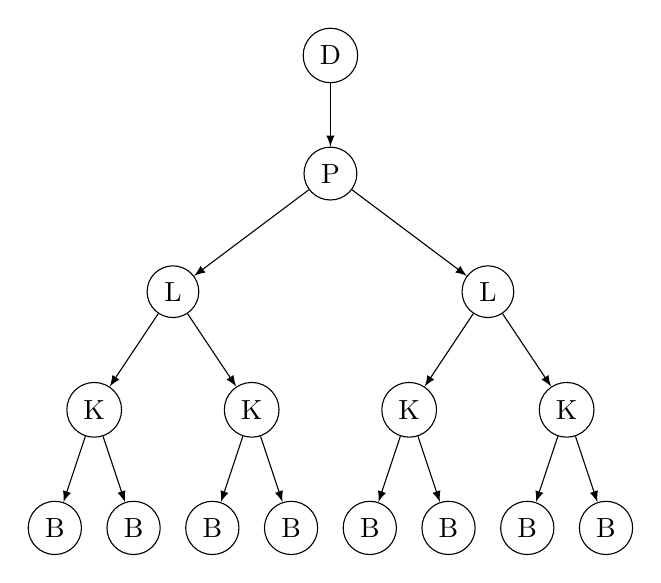
\begin{tikzpicture}[
    level 1/.style={sibling distance=40mm},
    level 3/.style={sibling distance=20mm},
    level 4/.style={sibling distance=10mm},
    every node/.style={draw,circle},
    arrow/.style={edge from parent/.style={draw,-latex}}
  ]
  \node {D}
      child[arrow] { node{P}
          child { node{L}
              child { node{K}
                  child {node{B}}
                  child {node{B}}
              }
              child { node{K}
                  child {node{B}}
                  child {node{B}}
              }
          }
          child { node{L}
              child { node{K}
                  child {node{B}}
                  child {node{B}}
              }
              child { node{K}
                  child {node{B}}
                  child {node{B}}
              }
          }
      }
  ;
  \end{tikzpicture}
  \caption{Illustrerer princippet bag, hvordan lampen overføres mellem de fem interessenter designer(D), producent(P), lampebutik(L), kunde(K) og bruger(B).}
  \label{fig:interessenter}
\end{figure}
% Sælgeren bliver også indirekte ramt, hvis mange kunder henvender sig fordi de gerne vil have en lampe returneret og byttet, så kræver det ressourcer fra lampebutikkers side. Derfor vil det også være til lampebutikkers fordel, at en kunde vil være i stand til at købe "den rigtige" lampe første gang eller en lampe, der er lidt dyrere fordi den giver den ønskede effekt.

\subsubsection{Designere}
Designere er interesseret i at deres design bliver solgt og er derfor sandsynligvis interesseret i et program, der kan hjælpe dem med at gøre deres design mere populært.

 
Vi har haft kontakt med to forskellige lampedesignere, danske Erik Mortensen, og svenske David Wahl fra IKEA. De sagde følgende:
\begin{center}
\textit{"I alle mine lamper er valg af lyskilde og placering sket på grundlag af test via prototyper. De fleste af mine lamper er prototyper"}.

\textit{"Jeg har i en del år arbejdet med lampedesign. og har derfor mest været optaget af armaturets/lampens skulpturelle udtryk, men da det jo er en lampe skal den selvfølgelig  også opfylde det belysningsmæssige."} Mailen kan ses i bilag \ref{sec:mailErik}.
\end{center}
og
\begin{center}
\textit{"Apart from hand sketching and physical prototypes, we use the 3D modeling application Solid Works in IKEA of Sweden. And for renderings we use either the built in renderer, or photo works, which is also part of solid works."} Mailen kan ses i bilag \ref{sec:mailDavid}.
\end{center}

Her er to eksempler på forskellige måder for designere, at visualisere en lampes lys på. Erik Mortensen benytter sig kun af prototyper, hvorudfra han kan se, hvordan lyset falder, hvorimod David Wahl, udover prototyper, også benytter sig af computerprogrammet Solid Works, til at visualisere lampens lys. 

\subsubsection{Producenter}
Producenten samarbejder med designeren om at udvikle lampen. Producentens rolle er at fremstille lampen på baggrund af designet. Når lamperne er produceret sendes de ud til lampebutikkerne. Producenten har en interesse i, at kunderne køber deres produkter i lampebutikkerne, da der er mulighed for, at dette vil medføre at lampebutikkerne bestiller flere af deres produkter hjem. En belysningskonsulent som vi har været i kontakt med, siger følgende om producenternes interesse i problemet: \textit{"Det er blevet en kompliceret proces at producere en lampe ift. EU lovgivning i dag så jeg har svært ved at se at producenterne vil koste endnu flere penge til produkter til privatmarkedet som måske kun køber en lampe til 3000 kr. som ofte kun interesserer sig for den laveste pris og ikke den bedste service og rådgivning. Så producenters incitament til ligge investeringer hos privatkunder er meget begrænset."} Mailen kan ses i bilag \ref{sec:mailbelysning}. Lampekonsulenten mener altså at producenterne ikke vil smide en masse penge ind i privatmarkedet, da det ikke gavner dem økonomisk. 


\subsubsection{Lampebutikker}
Lampebutikken er interesseret i at sælge flest mulige lamper, da dette giver større indkomst for butikken. Derudover er butikken også interesseret i, at kunden køber den 'rigtige' lampe første gang, da butikken på denne måde undgår utilfredse kunder, som vil returnere lamperne. 

Derudover er det lampebutikken, som er den primære rådgiver for kunderne, når der skal købes en ny lampe, derfor vil det være oplagt, at lave et værktøj, som lampebutikker kan stille til rådighed for sine kunder, så det bliver lettere at visualisere en lampe og dens belysning.


 

\subsubsection{Kunder}
Kunden er interesseret i at visualisere hvordan lys udbreder sig fra en lampe, da dette vil hjælpe kunden med at afgøre hvordan lampen passer ind i en kontekst, og kunden kan derfor undgå fejlkøb. Dette er kunden interesseret i, da det i sidste ende vil gavne brugeren af lampen, hvis kunden er i stand til at købe en lampe som passer ind i konteksten. Fejlkøb kan føre til økonomiske konsekvenser, hvis fejlen først indses efter lampen er installeret og emballagen er brudt, så lampen ikke kan returneres.

\subsubsection{Brugere}
Det er brugerne der i sidste ende benytter sig af lamperne i deres hjem eller på deres arbejde. Dette gør brugerne til den gruppe af interessenter, som påvirkes direkte af problemet, da de må leve med konsekvenserne, som belysningen fra en lampe kan medføre \ref{sec:konsekvenser}. Dette kan bl.a.\ være kontorarbejdere i en virksomhed, som påvirkes, hvis lamperne på deres kontor ikke passer sammen med indretningen. Et andet eksempel på brugere, er hjemme i privaten, hvor der kan være mange forskellige typer lamper, som skal passe ind i hjemmet. Hvis en person i hjemmet bruger en lampe, som har en belysning, der ikke passer ind i hjemmet pga.\ manglende visualisering ved købet, så vil dette påvirke brugerne i hjemmet, da dårlig belysning kan have sundhedsmæssige konsekvenser \ref{sec:konsekvenser}.



\subsubsection{Målgruppen}
Som beskrevet i forrige afsnit, er det både designere, producenter, butikker, kunder og brugere, der påvirkes af problemet. Det er nu relevant at afgøre hvem problemløsningen retter sig mod, da dette danner grundlag for, hvordan løsningen skal udvikles og hvem der kan indrages i løsningen og udarbejdelsen af løsningsforslaget.

Som illustreret på \ref{fig:interessenter} er det lampebutikkerne, som har den direkte kontakt til kunderne og via kunderne en forbindelse til brugerne. Designere er fravalgt, da vi ud fra mails fra Wahl og Mortensen kan uddrage, at de allerede har værktøjer til at visualisere lys fra lamper, og som der ses på skitsen har designeren ikke nogle direkte kontakt til kunden eller brugeren. Man kunne forestille sig, at problemet kunne løses allerede fra producentens side. Ud fra korrespondance med en belysningskonsulent i en lampebutik er dette dog blevet afvist \ref{sec:mailbelysning}. Vi er blevet informeret om, at producenterne ikke er interesseret i at bruge ressourcer på at løse problemet, da det ikke gavner producenterne direkte. Derudover er det ikke producentens opgave at vejlede kunder til det bedste køb af lamper, dette er derimod lampebutikken opgave.

Hvis man retter problemløsningen mod lampebutikker, og laver en løsning der gør det muligt for kunder at visualisere lamperne bedre, er det sandsynligt at kunderne vil være mere tilfredse med deres lamper, da de har mulighed for at se lampens belysning inden købet. For lampebutikker kan dette betyde, at kunden ikke returnerer lige så mange lamper, og dette vil bidrage til øget kundetilfredshed, som i sidste ende gavner både lampebutikker og kunderne. Hvis kunden er i stand til at købe en lampe som passer ind i den korrekte kontekst vil dette tilfredsstille brugeren. 

\subsubsection*{Opsummering}
I afsnittet er der blevet argumenteret for, at det påvirker brugeren af lampen hvis kunden ikke kan visualisere hvordan lyset udspreder sig fra en lampe, og dette vil i sidste ende også påvirke lampebutikkerne. Derudover er der blevet argumenteret for, at det er mest fordelagtigt at rette løsningen mod lampebutikker, da det er lampebutikkerne, der rådgiver kunderne, som køber lampen for brugerne.

Dette afsnit er relevant i forhold til den senere problemformulering, da der er blevet argumenteret for hvem det er, som har problemet, samt hvilken målgruppe det senere produkt skal udvikles til.

\clearpage
\subsection{Problemets placering}
I dette afsnit undersøges der, hvor, og i hvilke situationer problemet opstår. Da problemet tager udgangspunkt i købet af lampen, beskrives der, hvordan købssituationen er, ved hhv.\ handel i fysiske butikker(detailhandel), og handel i internetbaserede butikker(e-handel). Ud fra disse undersøgelser sammenlignes detailhandel og e-handel, for at afgøre hvor problemet er størst, og derudfra vælge hvilken type af handel, som denne rapport ønsker at løse problemet indenfor.

\subsubsection{Detailhandel}
En fysisk butik er et sted, hvor kunderne selv skal komme hen, når de vil købe eller kigge på butikkens varer. En fysisk butik har et personale, som tager sig af butikkens kunder, og som besvarer deres mulige spørgsmål til butikkens varer. En fysisk butik er, grundet det ansatte personale og andre udgifter, dyr i omkostning. Dog viser en amerikansk undersøgelse, at 92\% af de udspurgte 1029 personer i undersøgelsen foretrækker de fysiske butikker, da man kan se og føle de varen selv og få direkte assistance om varen gennem en medarbejder \cite{fysisk_kontra_online}. Det var ikke muligt at finde en lignende rapport, der viste noget om danskernes meninger mht.\ om de foretrækker at føle den fysiske vare, før de køber den, men grundet kulturelle ligheder mellem USA og Danmark, har vi valgt at antage at en lignende tendens er gældende i Danmark.

I vores kontekst snakker vi om en hvilken som helst fysisk butik, der har med lampesalg at gøre. Den lampeinteresserede kunde, kommer ud i butikken, og leder f.eks.\ efter en ny væglampe til stuen. Problemet heri kan opstå ved, at der er adskillige forskellige lamper at vælge imellem, men ikke alle lamperne er tilsluttet og man har derfor ikke mulighed for, at se lampens belysning i rummet.

\label{sec:sammenligning_af_e_og_d}
Ved køb af lamper i den fysiske butik, er det ikke altid, at de lamper, som stilles frem til udstilling giver et realistisk billede af, hvordan lyset udbreder sig, da der ofte er mange lamper og lyskilder tæt samlet. Et andet problem er returretten. Returretten er ikke obligatorisk at have for fysiske butikker, så det er altså op til den enkelte butik/butikskæde, om de vælger at gøre det muligt at returnere en vare selvom den er uåbnet og stadig i original emballage \cite{fortrydelsesret}. Hvis kunden beslutter sig for en lampe, som ikke er tilsluttet, men regner med at den vil se godt ud på væggen i stuen, hvorefter det så viser sig, at lyset falder helt forkert, er det for sent, da lampen er pakket ud, og ledningen er blevet pillet ved. Lampen kan altså ikke byttes, og er ikke optimal i forhold til kundens stue. Der er mange butikker og butikskæder, som vælger at gøre det muligt for kunden at bytte en vare, hvis den stadig er i original emballage og med kvittering \cite{ikea_returret}, men det er ikke noget, som butikker er tvunget til at gøre, og med en lampe som eksempel kan man ikke tage den med hjem og "afprøve", da dette giver afkald på returretten.

\subsubsection{E-handel}
\label{sec:ehandel}
E-handel er elektronisk handel via internettet\cite{ddo_ehandel}. På internettet kan lampebutikker have såkaldte e-butikker, hvor kunder kan købe varer\cite{ddo_ebutik}. E-butikker er ofte udformet således, at kunden kan se billeder og informationer omkring lampebutikkens varer og derudfra kan kunden vælge at lægge varerne i en virtuel indkøbskurv, hvor kunden til sidst indtaster de nødvendige oplysninger for at købe og modtage varerne.

Blandt de mange forskellige varer, der sælges via e-butikker, er det her relevant at tale om e-handel med lamper. Nedenstående figur \ref{fig:e_handel_med_lamper} illustrerer princippet bag en lampesælgers salg af lampe til en kunde via en e-butik.

\begin{figure}[H]
  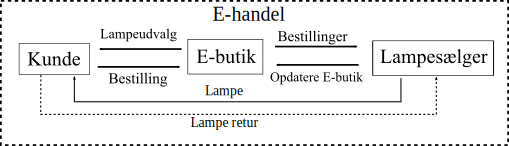
\includegraphics{e_handel_med_lampe.pdf}
  \caption{Princippet bag handel af en lampe via en e-butik.}
    \label{fig:e_handel_med_lamper}
\end{figure}

På figur \ref{fig:e_handel_med_lamper} er det vist, hvordan e-handlen starter med, at kunden får et udvalg af lamper fra e-butikken. Kunden sender så en bestilling, som via e-butikken sendes videre til lampebutikken, og til sidst sendes lampen til kunden. Dog ender handlen ikke nødvendigvis her, da kunden kan sende lampen retur såfremt at de gældende lovgivninger og købsbetingelser muliggør dette. For at undersøge lovgivningen nærmere kan man tage udgangspunkt i den danske lov om forbrugeraftaler\cite{retsinformationen}.

%
Lov om forbrugeraftaler

LOV nr 1457 af 17/12/2013 Gældende
(Forbrugeraftaleloven)
Offentliggørelsesdato: 18-12-2013
Justitsministeriet
%

I lovens kapitel 1, § 1, stk.\ 2, nr.\ 1 fremgår det, at lovens bestemmelser for fortrydelsesret gælder for aftaler, som er indgået ved fjernsalg. For en  fjernsalgsaftale gælder der, at aftalen om varer, er indgået gennem fjernkommunikation, hvor den erhvervsdrivende og forbrugeren ikke mødes fysisk (jf.\ kap. 1, § 3, nr.\ 1).

Ser man nu på loven i forbindelse med e-handel, foregår fjernkommunikationen gennem internettet via e-butikken, hvor fjernsalgsaftalen udføres i form af brugerens bestilling af f.eks.\ en lampe. Dette gør at fortrydelsesretten gælder ved e-handel.

Fortrydelsesretten er en kundes mulighed for at melde sig ud af en aftale, herunder køb af lamper ved e-handel. Hvis en kunde eksempelvis køber en lampe via en e-butik, har kunden mulighed for at fortryde købet inden 14 dage ved at meddele dette til den erhvervsdrivende (jf.\ kap.\ 4, § 19). Herefter har kunden 14 dage til at returnere varen (jf.\ kap.\ 4, § 24). Hvis varens værdi er forringet som følge af kundens unødvendige håndtering af varen for at inspicere denne, så hæfter kunden for værdiforringelsen (jf.\ kap.\ 4, § 24, stk.\ 5). Dvs.\ at hvis en bruger installerer og bruger lampen, hvor der f.eks.\ tilpasses ledninger, så kan lampens værdi forringes og kunden skal hæfte for dette. 


\subsubsection{Sammenligning af detail- og e-handel}
Ud fra ovenstående redegørelse af de to typer for handel, analyseres disse nu med henblik på at finde ligheder og forskelle, hvoraf det kan afgøres i hvilken af de to typer af handel, at problemet er størst. 

Da det initierende problem er, at kunden ikke kan visualisere lampen uden at købe den, er det derfor relevant, at se på i hvor høj grad dette er tilfældet ved de to typer handler.

Fordelen ved detailhandel er, at kunden ofte kan se lampen i butikken, og ud fra dette, vurdere hvilken lampe der opfylder de behov som kunden har \ref{sec:sammenligning_af_e_og_d}. Dog er problemet stadig, at kunden ikke ser lampen i den rette kontekst, dvs.\ i sit eget hjem. Dette kan gøre, at kunden får et godt indtryk af lampen i den kontekst, som butikken præsenterer den i, men at den ikke passer ind i den kontekst, som kunden køber lampen til.

Ved e-handel har kunden ikke muligheden for, at se en fysisk udgave af lampen, men ofte kun billeder. Dette gør at kunden alene kan tage valg ud fra de billeder og informationer som e-butikken præsenterer. Problemet er så, at billederne til dels ikke er interaktive, dvs.\ brugeren ikke kan se lampen fra flere vinkler end dem som billederne er taget i, samt at billederne ikke er taget af lampen i den kontekst, som kunden ønsker at købe lampen til. 

Med hensyn til konteksten er fordelen ved e-handel, at kunden kan sidde derhjemme, i den kontekst, hvor lampen skal indgå, og sammenligne med de informationer, der er tilgængelige på e-butikken. I modsætning til dette er detailbutikker, hvor kunden står i butikken, og måske har problemer med at huske eller blot forestille sig alle detaljerne ved den kontekst, som lampen skal indgå i.

Ud fra denne sammenligning, er der på den ene side detailhandel, hvor det er svært at visualisere konteksten, men hvor man kan se lampen. På den anden side er e-handel, hvor man kan sidde derhjemme i konteksten, men har svært ved at visualisere lampen. 

For at afgøre hvilken type handel denne rapport vil fokusere på, skal der derfor svares på om det er mangel på visualisering af lampen i kontekst ved detailhandel eller mangel på visualisering af lampen ved e-handel, som er det største problem.

Da kunden omgås og ser den kontekst, som lampen skal indgå i f.eks.\ et kontor, køkken og bad, må man kunne antage at kunden har en forestilling om, hvordan denne kontekst ser ud selvom kunden ikke står i den, når der handles i en fysisk butik. Derfor er dette ikke et lige så stort problem, som hvis kunden ikke kan visualisere lampen når der handles via e-handel. Derfor vil fokuset i denne rapport være at forbedre kundens evne til at visualisere lamper under e-handel.

\subsubsection*{Opsummering}
Ud fra ovenstående kan der opsummeres følgende iagttagelser for problemet i forhold til detail- og e-handel:
\begin{itemize}
\item Detailhandel: Fysisk lampebutik, hvor det kan være svært at visualisere lampen i den kontekst, som kunden vil købe lampen til, da kunden ikke er til stede derhjemme i konteksten.
\item E-handel: Internetbaseret lampebutik, hvor det kan være svært at visualisere lampen, som kunden vil købe, da kunden ikke kan se en fysisk udgave af lampen.
\end{itemize}
Ud fra ovenstående er valget faldet på visualisering af en lampe og dens belysning ved e-handel, da visualisering af selve lampen og dens belysning er højere prioritet end visualiseringen af den korrekte kontekst.

Dermed er der nu igennem problemanalysen afgrænset til, at det initierende problem skal løses ved sælgeren, herunder internetbaserede lampebutikker, hvor det er et problem at kunden mangler visualisering af lampen og dens belysning. Denne afgræsning samt problemanalysens resultater er opsummeret i den endelige problemformulering i næste afsnit.

\clearpage